\chapter{Cluster Creation}

Blablablabla

\section{Algorithm Configuration} \label{sssec:algo_config}

First of all, in the following section we will modify many times many files. As a rule, every time we modify a .cc or .h file, before launching the modified progroamm we will run

\begin{numVblock}\label{code:build}

\begin{verbatim}

cd $MY_TEST_AREA/WorkshopContent/build/
make install

\end{verbatim}
\end{numVblock}

If instead we modify a .xml, there is no need to run make install. In the following we will use many times files from the XmlHelper.h. For the pourpose of this guide, you do not need neither to modify nor to know this files, but in case you were curious you can find it in the Pandora Software Development Kit (PandoraSDK) located in:

\begin{verbatim}

$MY_TEST_AREA/PandoraPFA/PandoraSDK-v03-01-00/include/Helpers

\end{verbatim}

"The Pandora SDK aims to provide a robust, reliable and easy-to-use environment for developing and running pattern recognition algorithms" \cite{pandorasdk_paper}. The entire PandoraSDK can be found here \cite{pandora_doc}. 

At this point go in the folder

\begin{verbatim}

$MY_TEST_AREA/WorkshopContent/workshopcontent/Algorithms

\end{verbatim}

and open the files MyTestAlgorithm.h and MyTestAlgorithm.cc. Modify the .h file as it follows:

\begin{lstlisting}[language=C++, caption=Python example]

/**
 *  @file   WorkshopContent/workshopcontent/Algorithms/MyTestAlgorithm.h
 * 
 *  @brief  Header file for the mytest algorithm class.
 * 
 *  $Log: $
 */
#ifndef WORKSHOP_MYTEST_ALGORITHM_H
#define WORKSHOP_MYTEST_ALGORITHM_H 1

#include "Pandora/Algorithm.h"

namespace workshop_content
{

/**
 *  @brief  MyTestAlgorithm class
 */
class MyTestAlgorithm : public pandora::Algorithm
{
public:

	
    /**
     *  @brief  Factory class for instantiating algorithm
     */
  
 class Factory : public pandora::AlgorithmFactory
    {
    public:
        pandora::Algorithm *CreateAlgorithm() const;
    };

	/**
	*  @brief Defaul constructor
	*/
	MyTestAlgorithm();
private:
    pandora::StatusCode Run();
    pandora::StatusCode ReadSettings(const pandora::TiXmlHandle xmlHandle);

    // Member variables here

    std::string			m_myMandatoryString;		///< A mandatory string
    bool 			m_myOptionalBool;		///< An optional Boolean
    unsigned int		m_myOptionalUnsignedInt;	///< An optional unsigned int
    pandora::FloatVector	m_myMandatoryFloatVector;	///< A mandatory vector of floats


};


inline pandora::Algorithm *MyTestAlgorithm::Factory::CreateAlgorithm() const
{
    return new MyTestAlgorithm();
}


} // namespace workshop_content

#endif // #ifndef WORKSHOP_MYTEST_ALGORITHM_H

\end{lstlisting}

Then modify the .cc file from this

\begin{lstlisting}[language=C++, caption=Python example]
/**
 *  @file   WorkshopContent/workshopcontent/Algorithms/MyTestAlgorithm.cc
 * 
 *  @brief  Implementation of the mytest algorithm class.
 * 
 *  $Log: $
 */

#include "Pandora/AlgorithmHeaders.h"

#include "workshopcontent/Algorithms/MyTestAlgorithm.h"

using namespace pandora;

namespace workshop_content
{

StatusCode MyTestAlgorithm::Run()
{
    // Algorithm code here

    return STATUS_CODE_SUCCESS;
}

//-----------------------------------------

StatusCode MyTestAlgorithm::ReadSettings(const TiXmlHandle /*xmlHandle*/)
{
    // Read settings from xml file here

    return STATUS_CODE_SUCCESS;
}

} // namespace workshop_content

\end{lstlisting}

To this


\begin{lstlisting}[language=C++, caption=Python example]

/**
 *  @file   WorkshopContent/workshopcontent/Algorithms/MyTestAlgorithm.cc
 * 
 *  @brief  Implementation of the mytest algorithm class.
 * 
 *  $Log: $
 */

#include "Pandora/AlgorithmHeaders.h"

#include "workshopcontent/Algorithms/MyTestAlgorithm.h"

using namespace pandora;



namespace workshop_content
{

MyTestAlgorithm::MyTestAlgorithm() :
    m_myMandatoryString(),
    m_myOptionalBool(false),
    m_myOptionalUnsignedInt(5),
    m_myMandatoryFloatVector()
{
}
//---------------------------------
StatusCode MyTestAlgorithm::Run()
{
    std::cout	<<	"-m_myMandatoryString: " 	<< m_myMandatoryString 		<< std::endl
		<<      "-m_myOptionalBool: "	 	<< m_myOptionalBool    		<< std::endl
		<<	"-m_myOptionalUnsignedInt: "	<< m_myOptionalUnsignedInt	<< std::endl
		<<	"-m_myMandatoryString: ";	

    for (const auto value: m_myMandatoryFloatVector)
        std::cout << value << " ";    

    std::cout << std::endl;
    return STATUS_CODE_SUCCESS;
}

//--------------------------------

StatusCode MyTestAlgorithm::ReadSettings(const TiXmlHandle xmlHandle)
{
	PANDORA_RETURN_RESULT_IF(STATUS_CODE_SUCCESS, !=, XmlHelper::ReadValue(xmlHandle,"MyMandatoryString", m_myMandatoryString));
	PANDORA_RETURN_RESULT_IF_AND_IF(STATUS_CODE_SUCCESS, STATUS_CODE_NOT_FOUND, !=, XmlHelper::ReadValue(xmlHandle,"MyOptionalBool", m_myOptionalBool));
	PANDORA_RETURN_RESULT_IF_AND_IF(STATUS_CODE_SUCCESS, STATUS_CODE_NOT_FOUND, !=, XmlHelper::ReadValue(xmlHandle,"MyOptionalUnsignedInt", m_myOptionalUnsignedInt));
	PANDORA_RETURN_RESULT_IF(STATUS_CODE_SUCCESS, !=, XmlHelper::ReadVectorOfValues(xmlHandle,"MyMandatoryFloatVector", m_myMandatoryFloatVector));

        return STATUS_CODE_SUCCESS;
}

} // namespace workshop_content


\end{lstlisting}

These are actually basic modifications, but instructive to understand how the .cc file works. We will analyse now what these modifications mean and do.
\begin{lstlisting}[language=C++, caption=Python example]

MyTestAlgorithm::MyTestAlgorithm() :
    m_myMandatoryString(),
    m_myOptionalBool(false),
    m_myOptionalUnsignedInt(5),
    m_myMandatoryFloatVector()
{
}

\end{lstlisting}

simply assignes default values upon construction.

\begin{lstlisting}[language=C++, caption=Python example]
StatusCode MyTestAlgorithm::Run()
{
    std::cout	<<	"-m_myMandatoryString: " 	<< m_myMandatoryString 		<< std::endl
		<<      "-m_myOptionalBool: "	 	<< m_myOptionalBool    		<< std::endl
		<<	"-m_myOptionalUnsignedInt: "	<< m_myOptionalUnsignedInt	<< std::endl
		<<	"-m_myMandatoryString: ";	

    for (const auto value: m_myMandatoryFloatVector)
        std::cout << value << " ";    

    std::cout << std::endl;
    return STATUS_CODE_SUCCESS;
}
\end{lstlisting}

prints out the values at run time and

\begin{lstlisting}[language=C++, caption=Python example]
StatusCode MyTestAlgorithm::ReadSettings(const TiXmlHandle xmlHandle)
{
	PANDORA_RETURN_RESULT_IF(STATUS_CODE_SUCCESS, !=, XmlHelper::ReadValue(xmlHandle,"MyMandatoryString", m_myMandatoryString));
	PANDORA_RETURN_RESULT_IF_AND_IF(STATUS_CODE_SUCCESS, STATUS_CODE_NOT_FOUND, !=, XmlHelper::ReadValue(xmlHandle,"MyOptionalBool", m_myOptionalBool));
	PANDORA_RETURN_RESULT_IF_AND_IF(STATUS_CODE_SUCCESS, STATUS_CODE_NOT_FOUND, !=, XmlHelper::ReadValue(xmlHandle,"MyOptionalUnsignedInt", m_myOptionalUnsignedInt));
	PANDORA_RETURN_RESULT_IF(STATUS_CODE_SUCCESS, !=, XmlHelper::ReadVectorOfValues(xmlHandle,"MyMandatoryFloatVector", m_myMandatoryFloatVector));

        return STATUS_CODE_SUCCESS;
}
\end{lstlisting}
adds the optional and mandatory reads.

Now, try to run the program. As explained above, before running the program compile everything (in this guide, we will use the verb to compile and to build as synonyms):


\begin{verbatim}

cd $MY_TEST_AREA/WorkshopContent/build
make install

\end{verbatim}



At this point, you can try to run the program with:
\begin{numVblock}\label{code:launch}
\begin{verbatim}
$MY_TEST_AREA/WorkshopContent/bin/PandoraWorkshop                      \
-i $MY_TEST_AREA\WorkshopContent/settings/PandoraSettings_Workshop.xml \
-n 10
\end{verbatim}
\end{numVblock}
and you will get this error:

\begin{lstlisting}[language=Basic, caption=Python example]
XmlHelper::ReadValue(xmlHandle,"MyMandatoryString", m_myMandatoryString) return STATUS_CODE_NOT_FOUND
    in function: ReadSettings
    in file:     /usera/sv408/WorkshopContent/workshopcontent/Algorithms/MyTestAlgorithm.cc line#: 46
pLocalAlgorithm->ReadSettings(TiXmlHandle(pXmlElement)) throw STATUS_CODE_NOT_FOUND
    in function: CreateAlgorithm
    in file:     /usera/sv408/PandoraPFA/PandoraSDK-v03-01-00/src/Managers/AlgorithmManager.cc line#: 135
Failure in reading pandora settings, STATUS_CODE_NOT_FOUND
PandoraApi::ReadSettings(*pPandora, parameters.m_pandoraSettingsFile) throw STATUS_CODE_FAILURE
    in function: main
    in file:     /usera/sv408/WorkshopContent/workshopcontent/Test/PandoraWorkshop.cc line#: 88
Pandora Exception caught: STATUS_CODE_FAILURE
\end{lstlisting}

This is because we modified in the .cc file parts which needed the .xml without then modifiyng the .xml file. Therefore, open the .xml file 

\begin{verbatim}
$MY_TEST_AREA/WorkshopContent/settings	/PandoraSettings_Workshop.xml
\end{verbatim}

and where where you added (see Section \ref{sssec:new_algorithm}):

\begin{lstlisting}[language=XML]
  <algorithm type = "MyTestAlgorithm"/>
\end{lstlisting}

change and add the following lines:

\begin{lstlisting}[language=XML, caption=XML example]
   <algorithm type = "MyTestAlgorithm">
         <MyMandatoryString>TestString</MyMandatoryString>
	 <MyOptionalUnsignedInt>10</MyOptionalUnsignedInt>
         <MyMandatoryFloatVector>0. 1.5 3.0 4.5</MyMandatoryFloatVector>
    </algorithm>
\end{lstlisting}

At this point, run again the program with 
\begin{verbatim}
$MY_TEST_AREA/WorkshopContent/bin/PandoraWorkshop                      \
-i $MY_TEST_AREA\WorkshopContent/settings/PandoraSettings_Workshop.xml \
-n 10
\end{verbatim}

and you will see that in the output will appear also

\begin{lstlisting}[language=Basic, caption=Python example]
> Running Algorithm: Alg0001, LArEventReading
> Running Algorithm: Alg0002, LArListPreparation
> Running Algorithm: Alg0003, MyTestAlgorithm
-m_myMandatoryString: TestString
-m_myOptionalBool: 0
-m_myOptionalUnsignedInt: 10
-m_myMandatoryString: 0 1.5 3 4.5 
...
\end{lstlisting}

Therefore, even if very small, we managed to write and make it work a first simple Pandora algorithm.

\subsection{Application Programming Interfaces} \label{sssec:api}

"An API (application programming interface) is a term meaning the functions/methods in a library that you can call to ask it to do things for you - the interface to the library." \cite{stack_basics}. An API is basically something we do not need to modify that is an intermediate between us and libraries. We can use an API to call functions in the library without actually knowing exactly how this libriray works or it is made. If interested in seeing of an API is made, have a look to:

\begin{verbatim}
$MY_TEST_AREA/workshop/PandoraPFA/PandoraSDK-v03-01-00/include/Api/PandoraContentApi.h 
\end{verbatim}

\section{Adding a Sorting Algorithm} \label{sssec:sorting}

Now we want to change MyTestAlgorithm.cc and to start doing something a bit more elaborated. We want to take the fist n hits and sort them according to the z distance, which in 3D is given by the following formula:

\begin{equation}\label{eq:distance}
D=\sqrt{x^2+y^2+z^2}
\end{equation}

Modify the code MyTestAlgorithm.cc as it follows:

\begin{lstlisting}[language=C++, caption=Version of MyTestAlgorithms.cc to sort hits regarding z-coordinate]
/**
 *  @file   WorkshopContent/workshopcontent/Algorithms/MyTestAlgorithm.cc
 * 
 *  @brief  Implementation of the mytest algorithm class.
 * 
 *  $Log: $
 */

#include "Pandora/AlgorithmHeaders.h"

#include "larpandoracontent/LArHelpers/LArClusterHelper.h"

#include "workshopcontent/Algorithms/MyTestAlgorithm.h"

using namespace pandora;
using namespace lar_content;

namespace workshop_content
{
StatusCode MyTestAlgorithm::Run()
{

	const CaloHitList *pCaloHitList(nullptr);
	PANDORA_RETURN_RESULT_IF(STATUS_CODE_SUCCESS, !=, PandoraContentApi::GetCurrentList(*this, pCaloHitList));
	
	CaloHitVector sortedCaloHits(pCaloHitList->begin(), pCaloHitList->end());
	std::sort(sortedCaloHits.begin(), sortedCaloHits.end(), LArClusterHelper::SortHitsByPosition);

	for(const CaloHit *const pCaloHit : sortedCaloHits)
	{
		std::cout << "InputHit - HitType: " << pCaloHit->GetHitType() << ", " << pCaloHit->GetPositionVector() << std::endl;
	}

return STATUS_CODE_SUCCESS;



}



StatusCode MyTestAlgorithm::ReadSettings(const TiXmlHandle) //xmlHandle)
{


        return STATUS_CODE_SUCCESS;
}
}
\end{lstlisting}

and MyTestAlgorithm.h as well:

\begin{lstlisting}[language=C++, caption=Version of MyTestAlgorithms.h to sort hits regarding z-coordinate]
/**
 *  @file   WorkshopContent/workshopcontent/Algorithms/MyTestAlgorithm.h
 * 
 *  @brief  Header file for the mytest algorithm class.
 * 
 *  $Log: $
 */
#ifndef WORKSHOP_MYTEST_ALGORITHM_H
#define WORKSHOP_MYTEST_ALGORITHM_H 1

#include "Pandora/Algorithm.h"

namespace workshop_content
{

/**
 *  @brief  MyTestAlgorithm class
 */
class MyTestAlgorithm : public pandora::Algorithm
{
public:
    /**
     *  @brief  Factory class for instantiating algorithm
     */
  
 class Factory : public pandora::AlgorithmFactory
    {
    public:
        pandora::Algorithm *CreateAlgorithm() const;
    };
private:
    pandora::StatusCode Run();
    pandora::StatusCode ReadSettings(const pandora::TiXmlHandle xmlHandle);

    // Member variables here
};

inline pandora::Algorithm *MyTestAlgorithm::Factory::CreateAlgorithm() const
{
    return new MyTestAlgorithm();
}

} // namespace workshop_content

#endif // #ifndef WORKSHOP_MYTEST_ALGORITHM_H
\end{lstlisting}

Now, after building it as in code \ref{code:build}, run it using \ref{code:launch} and this is the outcome:

\begin{lstlisting}[language=Basic, caption=Python example]
> Running Algorithm: Alg0001, LArEventReading
> Running Algorithm: Alg0002, LArListPreparation
> Running Algorithm: Alg0003, MyTestAlgorithm
InputHit - HitType: 6,   x: 220.64  y: 0  z: 300.85 length: 373.086
InputHit - HitType: 6,   x: 220.659  y: 0  z: 301.15 length: 373.339
InputHit - HitType: 6,   x: 220.645  y: 0  z: 301.45 length: 373.572
InputHit - HitType: 6,   x: 220.642  y: 0  z: 301.75 length: 373.813
InputHit - HitType: 6,   x: 220.638  y: 0  z: 302.05 length: 374.052
InputHit - HitType: 6,   x: 220.645  y: 0  z: 302.35 length: 374.299
InputHit - HitType: 6,   x: 220.634  y: 0  z: 302.65 length: 374.535
InputHit - HitType: 6,   x: 220.581  y: 0  z: 302.95 length: 374.746
InputHit - HitType: 6,   x: 220.557  y: 0  z: 303.25 length: 374.974
InputHit - HitType: 6,   x: 220.556  y: 0  z: 303.55 length: 375.217
InputHit - HitType: 6,   x: 220.527  y: 0  z: 303.85 length: 375.442
InputHit - HitType: 6,   x: 220.189  y: 0  z: 304.15 length: 375.487
InputHit - HitType: 6,   x: 220.76  y: 0  z: 304.15 length: 375.822
InputHit - HitType: 6,   x: 220.13  y: 0  z: 304.45 length: 375.695
InputHit - HitType: 6,   x: 220.754  y: 0  z: 304.45 length: 376.061
...
\end{lstlisting}

Having a look to the outcome, we see InputHit - HitType. If we want to know what it means, we can do an useful exercise. Go to the PandoraSDK \cite{pandora_doc}, click on include and then objects. We are working with CaloHit, therefore click on CaloHit and search for HitType. You will find:

\begin{lstlisting}[language=C++]
 const HitType m_hitType; ///< The type of calorimeter hit
\end{lstlisting}

Now if you want to know what to what the number 6 is related, go to include, Pandora and PandoraEnumeratedTypes.h. Search again for HitType and you will find:

\begin{lstlisting}[language=C++]

/**
 *  @brief  Calorimeter hit type enum
 */
enum HitType
{
    TRACKER,
    ECAL,
    HCAL,
    MUON,
    TPC_VIEW_U,
    TPC_VIEW_V,
    TPC_VIEW_W,
    TPC_3D,
    HIT_CUSTOM
};
\end{lstlisting}
Keep in mind it starts counting from 0.

\section{Adding MCParticle List} \label{sssec:mcparticle_list}

Monte Carlo Particle list (MCParticle list) provides details of true pattern-recognition solition. This means that we start with simulated Monte Carlo (MC) events, than we reconstruct them and eventually we can check with MCParticle how good we have reconstruced those events. We will not us MCParticle for real data but it is really useful during the development process. We can now modify the MyTestAlgorithm.cc to add MCParticle as an output:

\begin{lstlisting}[language=C++, caption= MyTestAlgorithm.cc including for the first time MCParticles,label=code:mcpart_first]
/**
 *  @file   WorkshopContent/workshopcontent/Algorithms/MyTestAlgorithm.cc
 *  @brief  Implementation of the mytest algorithm class.
 */

#include "Pandora/AlgorithmHeaders.h"
#include "larpandoracontent/LArHelpers/LArClusterHelper.h"
#include "larpandoracontent/LArHelpers/LArMCParticleHelper.h"
#include "workshopcontent/Algorithms/MyTestAlgorithm.h"

using namespace pandora;
using namespace lar_content;

namespace workshop_content
{
StatusCode MyTestAlgorithm::Run()
{
	//CaloHits
	const CaloHitList *pCaloHitList(nullptr);
	PANDORA_RETURN_RESULT_IF(STATUS_CODE_SUCCESS, !=, PandoraContentApi::GetCurrentList(*this, pCaloHitList));
	
	CaloHitVector sortedCaloHits(pCaloHitList->begin(), pCaloHitList->end());
	std::sort(sortedCaloHits.begin(), sortedCaloHits.end(), LArClusterHelper::SortHitsByPosition);

	for(const CaloHit *const pCaloHit : sortedCaloHits)
	{
		std::cout << "InputHit - HitType: " << pCaloHit->GetHitType() << ", " << pCaloHit->GetPositionVector() << std::endl;
	}
	//MCParticle
	const MCParticleList *pMCParticleList(nullptr);
	PANDORA_RETURN_RESULT_IF(STATUS_CODE_SUCCESS, !=, PandoraContentApi::GetCurrentList(*this, pMCParticleList));

	MCParticleVector sortedMCParticles(pMCParticleList->begin(), pMCParticleList->end());
	std::sort(sortedMCParticles.begin(), sortedMCParticles.end(), LArMCParticleHelper::SortByMomentum);

	for (const MCParticle *const pMCParticle : sortedMCParticles)
	{
		std::cout << "InputMCParticle - PDG: " << pMCParticle->GetParticleId() << ", nParents " << pMCParticle->GetParentList().size()
			  << ", nDaughters " << pMCParticle->GetDaughterList().size() << std::endl;
	}
return STATUS_CODE_SUCCESS;

}

StatusCode MyTestAlgorithm::ReadSettings(const TiXmlHandle) //xmlHandle)
{


        return STATUS_CODE_SUCCESS;
}
}
\end{lstlisting}

and the output will be:

\begin{lstlisting}[language=Basic, caption=Output of the programm]
...
InputMCParticle - PDG: 2212, nParents 0, nDaughters 0
InputMCParticle - PDG: 13, nParents 0, nDaughters 0
InputMCParticle - PDG: 11, nParents 0, nDaughters 0
InputMCParticle - PDG: 11, nParents 0, nDaughters 0
InputMCParticle - PDG: 11, nParents 0, nDaughters 0
InputMCParticle - PDG: 11, nParents 0, nDaughters 0
InputMCParticle - PDG: 11, nParents 0, nDaughters 0
InputMCParticle - PDG: 11, nParents 0, nDaughters 0
InputMCParticle - PDG: 11, nParents 0, nDaughters 0
InputMCParticle - PDG: 11, nParents 0, nDaughters 0
InputMCParticle - PDG: 11, nParents 0, nDaughters 0
InputMCParticle - PDG: 11, nParents 0, nDaughters 0
InputMCParticle - PDG: 11, nParents 0, nDaughters 0
InputMCParticle - PDG: 11, nParents 0, nDaughters 0
InputMCParticle - PDG: 22, nParents 0, nDaughters 0
InputMCParticle - PDG: 22, nParents 0, nDaughters 0
...
\end{lstlisting}

Particle Data Group (PDG) is a number used to identify particles according to this table:
\begin{verbatim}
// Specify (name, pdg code, mass in GeV, width in GeV, charge)
#define PARTICLE_DATA_TABLE(d)                                                          \
    d(PHOTON,               22,             0.E+00f,             0.E+00f,       0)      \
    d(E_MINUS,              11,     5.10998902E-04f,             0.E+00f,      -1)      \
    d(E_PLUS,              -11,     5.10998902E-04f,             0.E+00f,      +1)      \
    d(MU_MINUS,             13,     1.05658357E-01f,        2.99591E-19f,      -1)      \
    d(MU_PLUS,             -13,     1.05658357E-01f,        2.99591E-19f,      +1)      \
    d(TAU_MINUS,            15,        1.77699E+00f,          2.265E-12f,      -1)      \
    d(TAU_PLUS,            -15,        1.77699E+00f,          2.265E-12f,      +1)      \
    d(NU_E,                 12,             0.E+00f,             0.E+00f,       0)      \
    d(NU_E_BAR,            -12,             0.E+00f,             0.E+00f,       0)      \
    d(NU_MU,                14,             0.E+00f,             0.E+00f,       0)      \
    d(NU_MU_BAR,           -14,             0.E+00f,             0.E+00f,       0)      \
    d(NU_TAU,               16,             0.E+00f,             0.E+00f,       0)      \
    d(NU_TAU_BAR,          -16,             0.E+00f,             0.E+00f,       0)      \
    d(PI_PLUS,             211,      1.3957018E-01f,         2.5284E-17f,      +1)      \
    d(PI_MINUS,           -211,      1.3957018E-01f,         2.5284E-17f,      -1)      \
    d(PI_ZERO,             111,       1.349766E-01f,            7.8E-09f,       0)      \
    d(LAMBDA,             3122,       1.115683E+00f,          2.501E-15f,       0)      \
    d(LAMBDA_BAR,        -3122,       1.115683E+00f,          2.501E-15f,       0)      \
    d(K_PLUS,              321,        4.93677E-01f,          5.315E-17f,      +1)      \
    d(K_MINUS,            -321,        4.93677E-01f,          5.315E-17f,      -1)      \
    d(K_SHORT,             310,        4.97672E-01f,          7.367E-15f,       0)      \
    d(K_LONG,              130,        4.97672E-01f,          1.272E-17f,       0)      \
    d(SIGMA_MINUS,        3112,         1.1975E+00f,           8.28E-15f,      -1)      \
    d(SIGMA_PLUS,         3222,         1.1975E+00f,           8.28E-15f,      +1)      \
    d(SIGMA_MINUS_BAR,   -3112,         1.1975E+00f,           8.28E-15f,      +1)      \
    d(SIGMA_PLUS_BAR,    -3222,         1.1975E+00f,           8.28E-15f,      -1)      \
    d(HYPERON_ZERO ,      3322,        1.31483E+00f,           2.28E-15f,       0)      \
    d(HYPERON_ZERO_BAR,  -3322,        1.31483E+00f,           2.28E-15f,       0)      \
    d(HYPERON_MINUS,      3312,        1.32131E+00f,           4.04E-15f,      -1)      \
    d(HYPERON_MINUS_BAR, -3312,        1.32131E+00f,           4.04E-15f,      +1)      \
    d(PROTON,             2212,      9.3827200E-01f,             0.E+00f,      +1)      \
    d(PROTON_BAR,        -2212,      9.3827200E-01f,             0.E+00f,      -1)      \
    d(NEUTRON,            2112,      9.3956533E-01f,          7.432E-28f,       0)      \
d(NEUTRON_BAR, -2112, 9.3956533E-01f, 7.432E-28f, 0)
\end{verbatim}

According to this table, in that particular event there were generated one protons, one muon, several electrons and photons.
\subsection{Enable Visualisation} \label{sssec:mcparticle_list_vis}

At this point, we want to modify Listing \ref{code:mcpart_first} in order to enable the visualisation. Modify as so MyTestAlgorithm.cc:

\begin{lstlisting}[language=C++, label=code:mcparticle_vis, caption=MyTestAlgorithm.cc now enables visualisation of both CaloHits (blue) and MCParticles (red)]
include "Pandora/AlgorithmHeaders.h"
#include "larpandoracontent/LArHelpers/LArClusterHelper.h"
#include "larpandoracontent/LArHelpers/LArMCParticleHelper.h"
#include "workshopcontent/Algorithms/MyTestAlgorithm.h"

using namespace pandora;
using namespace lar_content;

namespace workshop_content
{
StatusCode MyTestAlgorithm::Run()
{
	//CaloHits
	const CaloHitList *pCaloHitList(nullptr);
	PANDORA_RETURN_RESULT_IF(STATUS_CODE_SUCCESS, !=, PandoraContentApi::GetCurrentList(*this, pCaloHitList));
	
	const bool showDetectorGaps(true);
	PandoraMonitoringApi::SetEveDisplayParameters(this->GetPandora(), showDetectorGaps, DETECTOR_VIEW_XZ, -1.f, -1.f, 1.f);
	PandoraMonitoringApi::VisualizeCaloHits(this->GetPandora(), pCaloHitList, "CurrentCaloHits", BLUE);

	//MCParticle
	const MCParticleList *pMCParticleList(nullptr);
	PANDORA_RETURN_RESULT_IF(STATUS_CODE_SUCCESS, !=, PandoraContentApi::GetCurrentList(*this, pMCParticleList));
	PandoraMonitoringApi::VisualizeMCParticles(this->GetPandora(), pMCParticleList, "CurrentMCParticles", RED);

	PandoraMonitoringApi::ViewEvent(this->GetPandora());
return STATUS_CODE_SUCCESS;

}

StatusCode MyTestAlgorithm::ReadSettings(const TiXmlHandle) //xmlHandle)
{


        return STATUS_CODE_SUCCESS;
}
}
\end{lstlisting}

\begin{figure}[h]
\scalebox{1}{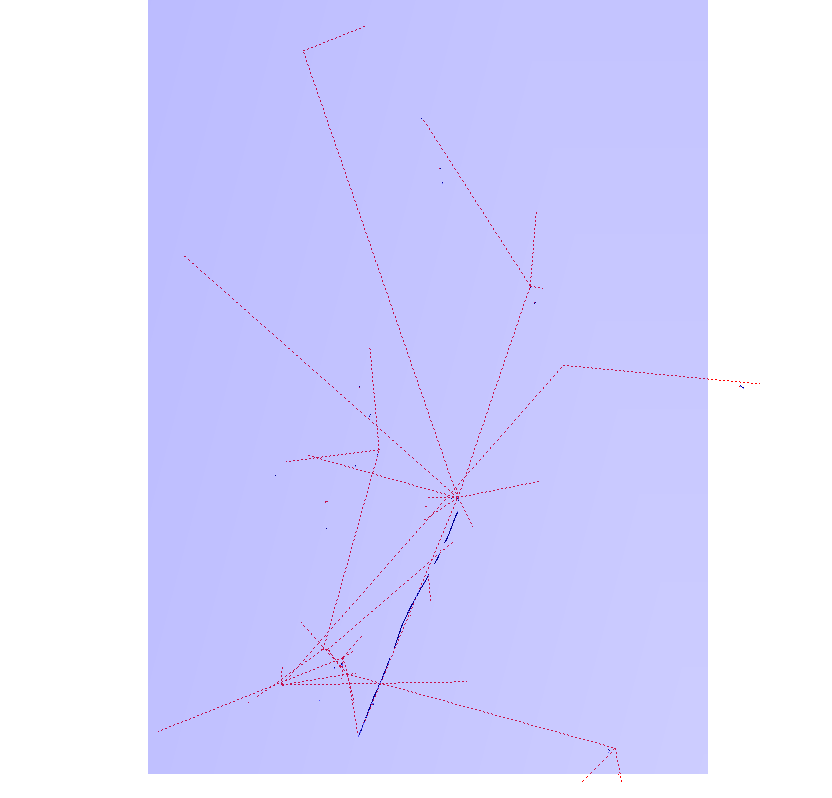
\includegraphics[width=0.5\textwidth]{/var/clus/usera/sv408/pandora_script/calo_and_mc}}
\centering
\caption{Pandora interface with CaloHits (blue) and MCParticles (red)}
\label{fig:calo_and_mc}
\end{figure}

From Figure \ref{fig:calo_and_mc} we can see the CaloHits and the MCParticles. For more examples, see 
\begin{verbatim}
$MY_TEST_AREA/WorkshopContent/examplecontent/ExampleAlgorithms/DisplayListsAlgorithm.cc or .h
\end{verbatim}

\section{Cluster Creationg} \label{sssec:cluster_creation}

A cluster is defined as

Modify MyTestAlgorithm.cc in this way:
\begin{lstlisting}[language=C++, label=code:first_cluster, caption=MyTestAlgorithm.cc creates a basic set of clusters]
#include "Pandora/AlgorithmHeaders.h"
#include "larpandoracontent/LArHelpers/LArClusterHelper.h"
#include "larpandoracontent/LArHelpers/LArMCParticleHelper.h"
#include "workshopcontent/Algorithms/MyTestAlgorithm.h"

using namespace pandora;
using namespace lar_content;

namespace workshop_content
{

MyTestAlgorithm::MyTestAlgorithm():
	m_outputClusterListName(),
	m_nHitsPerCluster(10)
	{
	}

StatusCode MyTestAlgorithm::Run()
{
	//CaloHits
	const CaloHitList *pCaloHitList(nullptr);
	PANDORA_RETURN_RESULT_IF(STATUS_CODE_SUCCESS, !=, PandoraContentApi::GetCurrentList(*this, pCaloHitList));
	
	const ClusterList *pTemporaryList(nullptr);
	std::string temporaryListName;
	PANDORA_RETURN_RESULT_IF(STATUS_CODE_SUCCESS, !=, PandoraContentApi::CreateTemporaryListAndSetCurrent(*this, pTemporaryList, temporaryListName));
	
	CaloHitVector sortedCaloHits(pCaloHitList->begin(), pCaloHitList->end());
	std::sort(sortedCaloHits.begin(), sortedCaloHits.end(), LArClusterHelper::SortHitsByPosition);

	const Cluster *pCluster(nullptr);
	
	for (const CaloHit *const pCaloHit : sortedCaloHits)
	{
		if (!PandoraContentApi::IsAvailable(*this, pCaloHit))
		    continue;
		if (!pCluster || (pCluster->GetNCaloHits() >= m_nHitsPerCluster))
		{
		   PandoraContentApi::Cluster::Parameters parameters;
                   parameters.m_caloHitList.push_back(pCaloHit);
		   PANDORA_RETURN_RESULT_IF(STATUS_CODE_SUCCESS, !=, PandoraContentApi::Cluster::Create(*this, parameters, pCluster));
		}
  		else
 		{
		  PANDORA_RETURN_RESULT_IF(STATUS_CODE_SUCCESS, !=, PandoraContentApi::AddToCluster(*this, pCluster, pCaloHit));
		}
	}
	if (!pTemporaryList->empty())
	{
	   PANDORA_RETURN_RESULT_IF(STATUS_CODE_SUCCESS, !=, PandoraContentApi::SaveList<Cluster>(*this, m_outputClusterListName));
	   PANDORA_RETURN_RESULT_IF(STATUS_CODE_SUCCESS, !=, PandoraContentApi::ReplaceCurrentList<Cluster>(*this, m_outputClusterListName));
	}
	return STATUS_CODE_SUCCESS;
}

StatusCode MyTestAlgorithm::ReadSettings(const TiXmlHandle xmlHandle)
	{
	  PANDORA_RETURN_RESULT_IF(STATUS_CODE_SUCCESS, !=, XmlHelper::ReadValue(xmlHandle, "OutputClusterListName", m_outputClusterListName));
	  PANDORA_RETURN_RESULT_IF_AND_IF(STATUS_CODE_SUCCESS, STATUS_CODE_NOT_FOUND, !=, XmlHelper::ReadValue(xmlHandle,"NHitsPerCluster", m_nHitsPerCluster));
	  return STATUS_CODE_SUCCESS;
	}

}
\end{lstlisting}

change also the MyTestAlgorithm.h

\begin{lstlisting}[language=C++, label=code:first_cluster.h, caption=MyTestAlgorithm.h]
#ifndef WORKSHOP_MYTEST_ALGORITHM_H
#define WORKSHOP_MYTEST_ALGORITHM_H 1

#include "Pandora/Algorithm.h"

namespace workshop_content
{

/**
 *  @brief  MyTestAlgorithm class
 */
class MyTestAlgorithm : public pandora::Algorithm
{
public:
    MyTestAlgorithm();
	
    /**
     *  @brief  Factory class for instantiating algorithm
     */
  
 class Factory : public pandora::AlgorithmFactory
    {
    public:
        pandora::Algorithm *CreateAlgorithm() const;
    };


	
private:
    pandora::StatusCode Run();
    pandora::StatusCode ReadSettings(const pandora::TiXmlHandle xmlHandle);

    // Member variables here

    std::string m_outputClusterListName;
unsigned int m_nHitsPerCluster;

};


inline pandora::Algorithm *MyTestAlgorithm::Factory::CreateAlgorithm() const
{
    return new MyTestAlgorithm();
}

} // namespace workshop_content

#endif // #ifndef WORKSHOP_MYTEST_ALGORITHM_H
\end{lstlisting}

and the PandoraSettings_Workshop.xml

\begin{lstlisting}[language=C++, label=code:first_cluster.xml, caption=PandoraSettings_Workshop.xml]
<pandora>
    <!-- GLOBAL SETTINGS -->
    <IsMonitoringEnabled>true</IsMonitoringEnabled>
    <ShouldDisplayAlgorithmInfo>true</ShouldDisplayAlgorithmInfo>
    <SingleHitTypeClusteringMode>true</SingleHitTypeClusteringMode>

    <!-- ALGORITHM SETTINGS -->
    <algorithm type = "LArEventReading">
        <EventFileNameList>/r05/uboone/jjd49/cincinatti_sample/Pandora_Events_Cincinatti_BNB_NuMu_1714.pndr</EventFileNameList>
        <GeometryFileName>/usera/sv408/WorkshopContent/settings/uboone/Geometry_MicroBooNE.xml</GeometryFileName>
        <SkipToEvent>0</SkipToEvent>
    </algorithm>

    <!-- LAR TPC EVENT RECONSTRUCTION -->
    <algorithm type = "LArListPreparation">
        <OnlyAvailableCaloHits>true</OnlyAvailableCaloHits>
        <OutputCaloHitListNameW>CaloHitListW</OutputCaloHitListNameW>
        <OutputCaloHitListNameU>CaloHitListU</OutputCaloHitListNameU>
        <OutputCaloHitListNameV>CaloHitListV</OutputCaloHitListNameV>
        <FilteredCaloHitListName>CaloHitList2D</FilteredCaloHitListName>
        <CurrentCaloHitListReplacement>CaloHitListW</CurrentCaloHitListReplacement>
        <OutputMCParticleListNameU>MCParticleListU</OutputMCParticleListNameU>
        <OutputMCParticleListNameV>MCParticleListV</OutputMCParticleListNameV>
        <OutputMCParticleListNameW>MCParticleListW</OutputMCParticleListNameW>
        <OutputMCParticleListName3D>MCParticleList3D</OutputMCParticleListName3D>
        <CurrentMCParticleListReplacement>MCParticleListW</CurrentMCParticleListReplacement>
        <MipEquivalentCut>0.</MipEquivalentCut>
    </algorithm>
<!-- parte nuova -->
   <algorithm type = "MyTestAlgorithm">
	<OutputClusterListName>MyFirstClusterW</OutputClusterListName>
    </algorithm>
<!-- fine parte nuova -->
    <algorithm type = "LArVisualMonitoring">
        <CaloHitListNames>CaloHitListW CaloHitListU CaloHitListV</CaloHitListNames>
        <MCParticleListNames>MCParticleList3D</MCParticleListNames>
        <SuppressMCParticles>22:0.01 2112:1.0</SuppressMCParticles>
        <ShowDetector>true</ShowDetector>
	<ClusterListNames>MyFirstClustersW</ClusterListNames>
    </algorithm>
</pandora>
\end{lstlisting}

Now we can understand how the code Listing \ref{code:first_cluster} works. The foundamental idea is that it takes the CaloHits, it sorts it in crescent order of z-coordinate, it than creates a cluster, it fills the cluster with the first 10 CaloHits, it then create a new cluster and re-iterate the process. 
\begin{lstlisting}[language=C++]
MyTestAlgorithm::MyTestAlgorithm():
	m_outputClusterListName(),
	m_nHitsPerCluster(10)
\end{lstlisting}
It defines and initialises variabiles, in particular says that m${\_}$nHitsPerCluster, the maximun number of CaloHits per cluster, is 10. 

\begin{lstlisting}[language=C++]
	const CaloHitList *pCaloHitList(nullptr);
	PANDORA_RETURN_RESULT_IF(STATUS_CODE_SUCCESS, !=, PandoraContentApi::GetCurrentList(*this, pCaloHitList));
\end{lstlisting}
In the first line you typedef CaloHitList std::list::<CaloHit>. So you define a new list of CaloHit named pCaloHitList and you initialise to zero. The second line says: "using PandoraContentApi, get from the file a list of CaloHits. If this operation is not success (the status code is different from the success status code) exit the program."

\begin{lstlisting}[language=C++]	
	const ClusterList *pTemporaryList(nullptr);
	std::string temporaryListName;
	PANDORA_RETURN_RESULT_IF(STATUS_CODE_SUCCESS, !=, PandoraContentApi::CreateTemporaryListAndSetCurrent(*this, pTemporaryList, temporaryListName));
\end{lstlisting}

First line same thing as before, creating a list of clusters named pTemporaryList. Third line you say: "using PandoraContentApi, create a new list and set it current. If it does not work, exit the programm".

\begin{lstlisting}[language=C++]
	CaloHitVector sortedCaloHits(pCaloHitList->begin(), pCaloHitList->end());
	std::sort(sortedCaloHits.begin(), sortedCaloHits.end(), LArClusterHelper::SortHitsByPosition);
\end{lstlisting}

It sorts CaloHits according to z coordinate.

\begin{lstlisting}[language=C++]
const Cluster *pCluster(nullptr);
\end{lstlisting}

It defines and initialises pCluster.

\begin{lstlisting}[language=C++]
	for (const CaloHit *const pCaloHit : sortedCaloHits)
	{
		if (!PandoraContentApi::IsAvailable(*this, pCaloHit))
		    continue;
\end{lstlisting}
For every CaloHit you have after been sorted. If you see that that CaloHit has already been counted, continue. In this case, continue means skip that CaloHit and go to the other one.
\begin{lstlisting}[language=C++]
		if (!pCluster || (pCluster->GetNCaloHits() >= m_nHitsPerCluster))
		{
		   PandoraContentApi::Cluster::Parameters parameters;
                   parameters.m_caloHitList.push_back(pCaloHit);
		   PANDORA_RETURN_RESULT_IF(STATUS_CODE_SUCCESS, !=, PandoraContentApi::Cluster::Create(*this, parameters, pCluster));
		}
  		else
 		{
		  PANDORA_RETURN_RESULT_IF(STATUS_CODE_SUCCESS, !=, PandoraContentApi::AddToCluster(*this, pCluster, pCaloHit));
		}
	}
\end{lstlisting}
If you do not have a cluster or the cluster is already filled with more CaloHits than the defined maximum number (in this case 10), create a new cluster and put CaloHit into it. Otherwise add to the cluster.
\begin{lstlisting}[language=C++]
	if (!pTemporaryList->empty())
	{
	   PANDORA_RETURN_RESULT_IF(STATUS_CODE_SUCCESS, !=, PandoraContentApi::SaveList<Cluster>(*this, m_outputClusterListName));
	   PANDORA_RETURN_RESULT_IF(STATUS_CODE_SUCCESS, !=, PandoraContentApi::ReplaceCurrentList<Cluster>(*this, m_outputClusterListName));
	}
	return STATUS_CODE_SUCCESS;
}
\end{lstlisting}
Quando hai finito la list, salvala.

\begin{lstlisting}[language=C++]
\end{lstlisting}

\begin{lstlisting}[language=C++]
\end{lstlisting}

